\subsection{La validation et le traitement des classeurs}
\label{subsec:spreadsheet-use-case}

\paragraph{}
Le coeur de l'application est la validation et le traitement des classeurs.
La validation vérifie que les données respectent les règles auxquelles elles doivent souscrire pour permettre l'usage auquel elles sont destinées.
Le traitement utilise les données et change l'état des bases de données des services qui vont consommer ces données.

\paragraph{}
Le travail que je présente ici est un \gls{g-framework}, une sorte de boite à outils conçut pour répondre à une gamme de besoins.
Il n'a donc pas d'utilité propre; on peut construire un banc avec une boite à outils et des planches, mais on ne peut pas s'assoir que sur le banc.
Les besoins auxquels doivent répondre ces outils, définis dans la sous-section \ref{subsec:business-needs}, sont des exemples venant d'applications propriétaires dont je ne peux pas discuter les spécifications exactes ici.
J'ai donc imaginé un exemple fictif qui a besoin des mêmes outils pour être satisfait.
Cet exemple aura aussi l'avantage de répondre à une logique métier beaucoup plus simple que les cas réels.
Pour rappel, vous pouvez consulter un exemple de cas réels dans l'annexe \ref{ch:leveltest-sample}.

\subsubsection{La validation d'un classeur}
\label{subsubsec:spreadsheet-validation-case}

\paragraph{}
Le classeur imaginé a deux feuilles, une qui contient des informations sur des apprenants et une sur des services.
Les apprenants sont des personnes pour lesquelles l'\textbf{utilisateur} veut créer des comptes pour qu'ils puissent suivre des cours sur nos plateformes.
Les services décrivent les accès que l'\textbf{utilisateur} veut donner à ces apprenants.

\begin{figure}[ht]
    \centering
    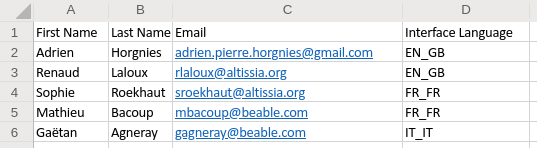
\includegraphics[width=0.7\textwidth]{images/screenshot/sheet-users.png}
    \caption{Un modèle valide de la feuille "registrants" qui liste les futurs apprenants}
    \label{fig:sheet-learners}
\end{figure}

\paragraph{}
Sur la figure \ref{fig:sheet-learners}, on peut voir les quatre attributs du futur élève:
\begin{itemize}
    \item First Name: Le prénom de l'apprenant est optionnel et s'il est présent, il doit être composé de lettres \gls{g-unicode} dont la première doit être une majuscule s'il existe une version majuscule de cette lettre\fnmark{}.
    \fntext{En réalité, il serait contraignant de limiter les noms à ce format tant la diversité est grande dans le monde. Ce cas n'est qu'un exemple d'utilisation d'une \gls{g-regex}}
    \item Last Name: Le nom de l'apprenant est obligatoire et respecte les mêmes règles que le prénom.
    \item Email: L'email est obligatoire, doit être un email valide et doit être unique dans la feuille.
    \item Interface language: La langue est obligatoire et doit faire partie d'une énumération définie par le code de l'application.
\end{itemize}

\paragraph{}
Voici un extrait pertinent du code qui définit les langues, dont vous pouvez lire l'entièreté dans l'annexe \ref{ch:language-java}:

\lstinputlisting[language=java, firstnumber=13, firstline=13, lastline=19]{pages/appendix/Language.java}

On y observe qu'il y a deux sortes de langues, les langues d'apprentissages et les langues d'études.
Une langue d'étude est implicitement aussi une langue d'interface.
Il est impératif de se servir de cette classe et non d'une copie, car il faut suivre ses évolutions.

\begin{figure}[ht]
    \centering
    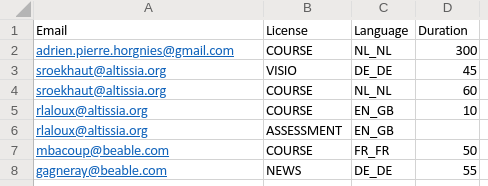
\includegraphics[width=0.7\textwidth]{images/screenshot/sheet-services.png}
    \caption{Un modèle valide de la feuille "services" qui liste les licences nécessaires aux apprenants}
    \label{fig:sheet-services}
\end{figure}

\paragraph{}
La feuille décrivant les services, dont un exemple est illustré par la figure \ref{fig:sheet-services}, contient les champs suivants:
\begin{itemize}
    \item Email: L'email est obligatoire et doit avoir été défini par un utilisateur sur l'autre feuille pour pouvoir être utilisé.
    \item License: La licence est obligatoire et doit être un membre de l'énumération \textit{Service} définie dans le code.
    \item Language: La langue est obligatoire, doit être une langue d'étude et donc faire partie d'un ensemble restreint de l'énumération \textit{Language}.
    \item Duration: Cette durée, exprimée en jours entiers, doit être comprise entre 0 et 365.
\end{itemize}
La classe \textit{Service} n'a rien de particulier et elle définit les éléments suivants: \textit{COURSE}, \textit{ASSESSMENT}, \textit{NEWS}, \textit{VISIO}.

La combinaison de l'email, la licence et la langue doivent être uniques dans la feuille.

\paragraph{}
Outre les règles au sein des feuilles, des règles sont appliquées sur l'ensemble du classeur:
\begin{itemize}
    \item Un email défini dans la feuille "registrants" doit être utilisé dans la feuille "services"
    \item Un email utilisé par la feuille des "services" doit être défini dans la feuille "registrants"
    \item Certaines erreurs peuvent être reclassées comme des avertissements, qui peuvent être ignorés pour procéder au traitement
\end{itemize}

\paragraph{}
Enfin, certaines règles sont externes au contenu du seul classeur:
Un email défini dans la feuille "registrants" ne peut pas être déjà présent dans la base des données des apprenants; l'apprenant doit être nouveau.

\subsubsection{Le traitement d'un classeur}
\label{subsubsec:spreadsheet-processing-case}

\begin{figure}[ht]
    \centering
    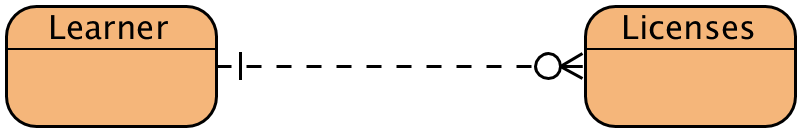
\includegraphics[width=0.7\textwidth]{images/diagrams/entity-relationship.png}
    \caption{Le diagramme entité-relation des deux entités utilisées pour la démonstration}
    \label{fig:entity-relationship}
\end{figure}

Le traitement de ce classeur consiste à créer les apprenants, leurs licences et les liens entre les deux à partir des informations contenues dans le classeur.
